% TechTronics — IEEE SP Cup 2027, Round 1 technical report (DRAFT, 27 Nov 2026)
% Build: pdflatex main && bibtex main && pdflatex main && pdflatex main  (or upload the zip to Overleaf)
% Every number comes from a script in the repository (source table + git hash in the comment next to it).
% Red \todo{}/TBD items are runs still in progress or text still to be written.
\documentclass[conference]{IEEEtran}
\usepackage[utf8]{inputenc}
\usepackage[T1]{fontenc}
\usepackage{amsmath,amssymb}
\usepackage{graphicx}
\usepackage{booktabs}
\usepackage{siunitx}
\usepackage{xcolor}
\usepackage{tikz}
\usetikzlibrary{positioning,arrows.meta}
\usepackage[hidelinks]{hyperref}
\usepackage{cite}

\newcommand{\todo}[1]{\textcolor{red}{[TODO: #1]}}
\newcommand{\tbd}{\textcolor{red}{TBD}}
\sisetup{detect-weight=true}

\begin{document}

\title{FaceVitals: SNR-Weighted Anatomical Multi-Patch Remote Photoplethysmography\\for Heart-Rate Estimation under Real-World Constraints}

\author{\IEEEauthorblockN{Muftee Mysan, Thamilezai Ananthakumar, Sulojan Rajkumar, Nadha Irshad, Rajinthan Rameshkumar,
John Praveen, Joshua Kulasingham}
\IEEEauthorblockA{Team TechTronics, University of Moratuwa, Sri Lanka\\
mufteemysan@gmail.com}}

\maketitle

\begin{abstract}
We present FaceVitals, a classical, fully explainable camera-based heart-rate (HR) pipeline for the IEEE SP Cup 2027.
MediaPipe landmarks place ten anatomically defined skin patches on the designated face; per patch, skin pixels are
averaged with a trimmed mean and denoised by a pixel-count-weighted Kalman filter; the pulse is extracted with the
plane-orthogonal-to-skin (POS) projection and band-passed; and in every 10\,s window the patch spectra are fused with
weights equal to their pulse signal-to-noise ratio (SNR). One configuration is used for all datasets. On the 30 held-out
UBFC-rPPG test subjects the pooled mean absolute error (MAE) is \SI{1.93}{bpm} (median per subject \SI{1.17}{bpm},
96\,\% of windows within \SI{5}{bpm}). On the demographically diverse AiPEX dataset (India and Sierra Leone) the test MAE
is \SI{5.96}{bpm} (95\,\% CI 4.2--7.9), on par with the best published method (\SI{5.8}{bpm}) and down from
\SIrange{14}{19}{bpm} for our initial pipelines, with equal error in both countries and no statistically significant
difference between skin-tone groups. All seven competition constraints are addressed with the official MATLAB recipes.
\end{abstract}

\begin{IEEEkeywords}
remote photoplethysmography, heart rate, POS, SNR fusion, Kalman filter, skin tone, edge computing
\end{IEEEkeywords}

% ================================================================================================
\section{Introduction}
Remote photoplethysmography (rPPG) estimates the blood-volume pulse from subtle colour changes of facial skin
recorded by an ordinary camera~\cite{dehaan2013chrom,wang2017pos}. Contact-free HR is attractive for telemedicine,
but accuracy degrades under low light, low resolution and bandwidth, motion, occlusion, bystanders, aging skin and
darker skin tones~\cite{dasari2021bias}. The SP Cup 2027 asks for HR estimation under controlled and uncontrolled
conditions with constraints C1--C7.

\textbf{Contributions.}
\begin{itemize}
  \item A single classical pipeline for all datasets: anatomical multi-patch selection~\cite{li2026roi}, trimmed-mean
        skin pooling, per-patch Kalman denoising and per-window SNR-weighted spectral fusion.
  \item A reproducible development protocol: frozen dev/test splits, 5-fold cross-validation, a pre-registered keep/reject
        rule (paired bootstrap), an experiment log of 22 hypotheses, and full disclosure of one post-freeze change.
  \item Fairness reporting (C2) with bootstrap confidence intervals, a permutation test and a country $\times$ skin-tone
        cross-tabulation instead of a pass/fail claim.
  \item A constraint suite C1--C7 on the official MATLAB recipes and a designated-target multi-face tracker (C3).
  \item An on-device web demonstrator, and a pulse-preserving video encoding for the submission package.
\end{itemize}

% ================================================================================================
\section{Related work}
Model-based rPPG projects normalised RGB traces onto pulse-sensitive directions: CHROM~\cite{dehaan2013chrom} uses
chrominance signals, POS~\cite{wang2017pos} a plane orthogonal to the skin tone. Region choice matters: the glabella,
nasal dorsum and malar regions are the most robust, and fusing the best few regions beats both a single region and the
whole face~\cite{li2026roi,bondarenko2025roi}. Constraining how fast HR may change improves robustness to spurious
peaks~\cite{tian2026correction}. Dasari \emph{et al.}~\cite{dasari2021bias} released AiPEX to quantify demographic bias;
the bounded Kalman filter (BKF)~\cite{prakash2018bkf} was the most accurate method on it. Agreement with a reference
device is assessed with Bland--Altman analysis rather than correlation alone~\cite{altman1983measurement,bland1986statistical}.
\todo{organiser group's prior work (Jeyakumar 2020/2022, Arulselvi 2023); aging skin (Caroppo 2024).}

% ================================================================================================
\section{Method}
Fig.~\ref{fig:pipeline} shows the frozen Round-1 configuration (CP3) and Table~\ref{tab:params} its parameters. The
pipeline is classical: the only learned components are pretrained face detectors/landmarkers; nothing is trained on HR data.

\begin{figure}[t]
\centering
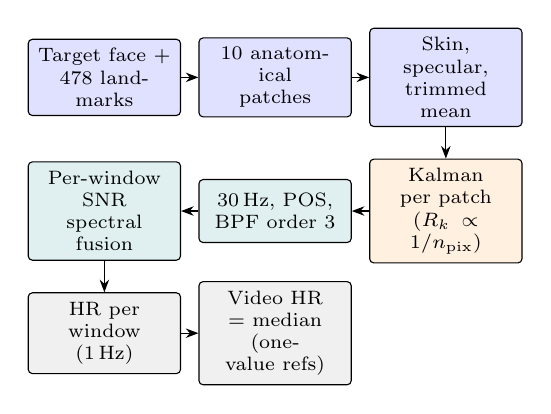
\begin{tikzpicture}[node distance=2.2mm and 2.2mm, font=\scriptsize,
  box/.style={draw, rounded corners=1.5pt, align=center, minimum height=8mm, text width=17mm, fill=#1!12},
  box/.default=gray, >={Stealth[length=1.6mm]}]
\node[box=blue] (lm) {Target face +\\478 landmarks};
\node[box=blue, right=of lm] (patch) {10 anatomical\\patches};
\node[box=blue, right=of patch] (pix) {Skin, specular,\\trimmed mean};
\node[box=orange, below=4mm of pix] (kal) {Kalman per patch\\($R_k\propto 1/n_{\mathrm{pix}}$)};
\node[box=teal, left=of kal] (pos) {30\,Hz, POS,\\BPF order 3};
\node[box=teal, left=of pos] (snr) {Per-window SNR\\spectral fusion};
\node[box=gray, below=4mm of snr] (hr) {HR per window\\(1\,Hz)};
\node[box=gray, right=of hr] (vid) {Video HR = median\\(one-value refs)};
\draw[->] (lm) -- (patch); \draw[->] (patch) -- (pix); \draw[->] (pix) -- (kal);
\draw[->] (kal) -- (pos); \draw[->] (pos) -- (snr); \draw[->] (snr) -- (hr); \draw[->] (hr) -- (vid);
\end{tikzpicture}
\caption{Frozen Round-1 pipeline (CP3). Blue: front end (input adapter); orange: denoising; green: signal chain.
For AiPEX the input adapter uses the three supplied crops as patches instead of the first two boxes.}
\label{fig:pipeline}
\end{figure}

\subsection{Target face, landmarks and anatomical patches (C3, C7)}
MediaPipe Face Landmarker~\cite{kartynnik2019facemesh} returns 478 landmarks for up to four faces per frame. The designated
target is the largest face at the start (or a user-selected face); afterwards the face nearest to the previous target is
followed and re-acquired only within half a face width, so bystanders are not adopted. Landmarks are smoothed with a
1-Euro filter~\cite{casiez2012oneeuro} (min.\ cutoff \SI{1}{Hz}, $\beta=0.02$). Ten patches are defined on the landmark
mesh exactly as published by Li~\emph{et al.}~\cite{li2026roi}: glabella, nasal dorsum, left/right malar (group A), medial and
lateral forehead (B), philtrum and left/right submalar (C). The multi-face tracker of our face module
(RetinaFace~\cite{deng2020retinaface}, a Kalman track per face, KLT~\cite{shi1994good}) is evaluated for C3/C4/C7 in
Section~\ref{sec:constraints}.

\subsection{Pixel selection and Kalman denoising}
Inside each patch, pixels inside a YCbCr skin box that are not specular ($Y\le0.95\cdot255$, no saturated channel) are
averaged with a 10\,\%/10\,\% trimmed mean; a patch is valid in a frame if at least 20 pixels remain. Each colour
channel of each patch is denoised on the native frame times by a Kalman filter with a random-walk level and measurement
noise $R_k = R_0\,\mathrm{median}(n)/n_k$, so frames averaged over fewer pixels are trusted less; the process noise places
the steady-state \SI{-3}{dB} point at $\min(\SI{4}{Hz}, 0.4 f_s)$, above the HR band.

\subsection{Pulse extraction and SNR-weighted spectral fusion}
Each patch trace is resampled to \SI{30}{Hz} using the measured frame timestamps, projected with POS~\cite{wang2017pos}
(\SI{1.6}{s} window, overlap-add) and band-passed with a zero-phase third-order Butterworth filter
(\SIrange{0.7}{3.0}{Hz}, \SIrange{42}{180}{bpm}). In every \SI{10}{s} window (\SI{1}{s} step) each patch with at least
90\,\% valid samples contributes a Hann-windowed periodogram $P_i(f)$ (8192-point FFT), normalised to unit power in the
band. Its SNR~\cite{dehaan2013chrom} is the power within \SI{\pm0.1}{Hz} of its in-band peak $f_0$ and \SI{\pm0.2}{Hz} of
$2f_0$, divided by the remaining in-band power (linear). The fused spectrum and the window HR are
\begin{equation}
  P(f) = \sum_i \mathrm{SNR}_i\,\frac{P_i(f)}{\int_{\mathrm{band}} P_i},\qquad
  \widehat{\mathrm{HR}} = 60\,\arg\max_f P(f).
\end{equation}
A patch with a weak or noisy pulse in a window (shadow, partial cover, low reflectance) therefore contributes little to
that window only. For datasets with one reference value per video (AiPEX) the video-level HR is the median of the window
HRs. This signal chain was developed independently by a team member in Python and ported to MATLAB for the reference
implementation (Section~\ref{sec:aipex}).

\subsection{Reference HR}
The contact PPG is interpolated onto the same \SI{30}{Hz} grid, detrended~\cite{tarvainen2002detrending} and band-passed, and its periodogram peak is
taken in the same windows; it never passes through fusion, Kalman filtering or tracking, so our errors are not understated.

\begin{table}[t]
\centering
\caption{Frozen Round-1 configuration (CP3, tag \texttt{round1-freeze-cp3}, 27 Nov 2026).}
\label{tab:params}
\begin{tabular}{@{}ll@{}}
\toprule
Landmarks / patches & MediaPipe 478 pts, 10 patches~\cite{li2026roi}, 1-Euro 1\,Hz, $\beta$ 0.02 \\
Pixels & YCbCr skin, specular removal, trimmed mean 10/10\,\% \\
Kalman (per patch) & $R_k\propto1/n_{\mathrm{pix}}$, \SI{-3}{dB} at $\min(4\,\mathrm{Hz}, 0.4f_s)$ \\
Resampling / POS & 30\,Hz linear / 1.6\,s \\
Band-pass & Butterworth order 3, 0.7--3.0\,Hz, zero phase \\
HR windows & 10\,s, step 1\,s, Hann periodogram, 8192-point FFT \\
Fusion & linear SNR weights ($\pm$0.1\,Hz peak, $\pm$0.2\,Hz harmonic) \\
Validity & $\ge20$ px per patch; $\ge90$\,\% valid samples per patch and window \\
Video-level HR & median of window HRs \\
\bottomrule
\end{tabular}
\end{table}

% ================================================================================================
\section{Datasets and protocol}
\textbf{UBFC-rPPG}~\cite{bobbia2019ubfc} (DATASET\_2): 42 subjects, $640\times480$, about 30\,fps, contact PPG.
\textbf{AiPEX}~\cite{dasari2021bias}: 44 subjects from India and 44 from Sierra Leone; per subject three pre-cropped ROI
videos (15\,fps) and one mean HR from a Masimo oximeter. Face detection is bypassed for AiPEX (input adapter only).
\textbf{Sri Ramachandra} (organiser data): no ground truth was supplied; it is never used for tuning or accuracy claims.

\textbf{Splits.} UBFC dev = subjects \{1, 3, 5, 8--16\}, test = the other 30. AiPEX is split by subject with a fixed seed
into dev (62) and test (26; 13 per country). Development used dev only: AiPEX with 5-fold cross-validation stratified by
country (nested for multi-valued settings); a change was kept only if the paired-bootstrap 95\,\% CI of its gain excluded
zero, UBFC-dev did not degrade by more than 0.1\,bpm and the India--Sierra Leone gap did not widen by more than 0.5\,bpm.

\textbf{Freeze and one disclosed change.} A first configuration (CP2) was frozen on 27 Nov 2026 and run on both test sets.
A team member's independently developed SNR-fusion chain was then found to be clearly better on AiPEX-dev (5.59 vs
\SI{8.82}{bpm}) and not worse on UBFC-dev (1.39 vs \SI{1.41}{bpm}); it was adopted and re-frozen as CP3, and both test
sets were run once more. Because the teammate chose that combination after seeing results on all AiPEX videos, and CP2
had already been scored on the test sets, AiPEX-test is not fully held out for CP3; we report both configurations.
The 42-subject UBFC numbers of our initial pipeline predate the split.

\textbf{Metrics.} MAE, RMSE, Pearson $r$, Bland--Altman bias and 95\,\% limits of agreement
(LoA)~\cite{bland1986statistical}, SUC@3/SUC@5 (share within 3/5\,bpm) and coverage; 10\,s windows with 1\,s step for UBFC,
one value per video for AiPEX. \todo{repeated-measures LoA and subject-level bootstrap CIs for UBFC.}

% ================================================================================================
\section{Results}
\label{sec:results}

\subsection{UBFC-rPPG}
% sources: outputs/repro/ubfc2_seeded_pooled.csv (318426d); outputs/ablation_roi/summary.csv (a275573);
%          outputs/round1/ubfc_{dev,test}_summary.csv (CP2), ubfc_{dev,test}_cp3_summary.csv (CP3; 3aee377)
\begin{table}[t]
\centering
\caption{UBFC-rPPG, pooled over 10\,s windows (bpm).}
\label{tab:ubfc}
\begin{tabular}{@{}lccccc@{}}
\toprule
Pipeline (subjects) & MAE & RMSE & $r$ & LoA & SUC@5 \\
\midrule
Initial: box regions (all 42)       & 2.17 & 6.49 & 0.936 & $-13.7$/$+11.4$ & -- \\
Box regions, SNR fusion (dev 12)    & 2.51 & 6.71 & 0.929 & -- & 92.7\,\% \\
CP2 (dev 12)                        & 1.41 & 2.34 & 0.991 & $-4.9$/$+4.2$ & 97.1\,\% \\
CP2 (test 30)                       & 1.46 & 4.66 & 0.967 & $-9.8$/$+8.2$ & 97.9\,\% \\
\textbf{CP3, frozen (dev 12)}       & \textbf{1.39} & \textbf{2.32} & \textbf{0.991} & $-4.9$/$+4.1$ & 96.5\,\% \\
\textbf{CP3, frozen (test 30)}      & \textbf{1.93} & \textbf{6.28} & \textbf{0.943} & $-13.3$/$+10.8$ & 96.1\,\% \\
\bottomrule
\end{tabular}
\end{table}

Table~\ref{tab:ubfc} shows that the anatomical patches are the decisive change on UBFC: with the same signal chain and
reference windows, moving from three box regions to the ten patches lowered the dev MAE from 2.51 to \SI{1.37}{bpm}.
On the 30 test subjects the frozen CP3 reaches a pooled MAE of \SI{1.93}{bpm} with a median per-subject MAE of
\SI{1.17}{bpm}; only one subject exceeds \SI{5}{bpm} (subject 48, \SI{10.2}{bpm}), which also widens the limits of
agreement. The superseded CP2 was better on this split (\SI{1.46}{bpm}); we keep CP3 because the choice between them was
made on dev data, and choosing on test results would bias the evaluation. Failure analysis of the initial pipeline
(Fig.~\ref{fig:persubject}) traced its worst subject (15, \SI{24.8}{bpm}) to a weak pulse combined with face-box jumps every
second when the Viola--Jones detector~\cite{viola2001rapid} re-ran; with smoothed landmark patches it falls to
\SI{1.9}{bpm}. Subjects 27, 41 and 49 showed bursts of error during head motion.

\begin{figure}[t]
\centering
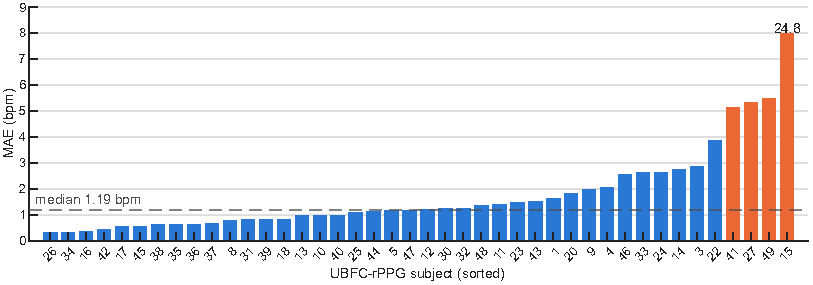
\includegraphics[width=\columnwidth]{figures/ubfc2_per_subject.pdf}
\caption{Per-subject MAE of the initial pipeline on all 42 UBFC subjects (POS, combined box region). Orange: MAE
$>5$\,bpm; bar for subject 15 clipped.}
\label{fig:persubject}
\end{figure}

\subsection{Constraints C1--C7}
\label{sec:constraints}
% source: face module run_pipeline @ 921910d, reproduced 26 Nov 2026 (docs/REPRODUCTION.md)
\textbf{Multi-face tracker under C3/C4/C7.} Degraded copies of UBFC were generated with the official recipes
(\texttt{imresize} bicubic to $320\times240$ for C4; a second, real pulsing subject composited beside the target for C3; a
filled \texttt{insertShape} polygon over the lower face for C7). On six held-out subjects (Table~\ref{tab:constraints}) the
target was tracked in every frame with no identity switch, and each constraint added less than \SI{0.2}{bpm}.
\begin{table}[t]
\centering
\caption{Multi-face tracker under constraints, subjects 3, 4, 12, 26, 31, 34 (POS baseline; MAE/RMSE averaged over subjects, bpm).}
\label{tab:constraints}
\begin{tabular}{@{}lccccc@{}}
\toprule
Condition & Target & ID sw. & MAE & RMSE & SUC@5 \\
\midrule
Baseline ($640\times480$) & 100\,\% & 0 & 1.28 & 2.14 & 96.8\,\% \\
C4 ($320\times240$)       & 100\,\% & 0 & 1.42 & 2.36 & 96.0\,\% \\
C3 (bystander)            & 100\,\% & 0 & 1.28 & 2.15 & 96.8\,\% \\
C7 (mask)                 & 100\,\% & 0 & 1.45 & 2.40 & 95.7\,\% \\
C3+C4+C7                  & 100\,\% & 0 & 1.48 & 2.47 & 95.3\,\% \\
\bottomrule
\end{tabular}
\end{table}

\textbf{Frozen pipeline under C1, C4, C5, C6, C7.} Pre-specified subset: UBFC test subjects 4, 17, 18, 20, first 30\,s.
C1: $\mathrm{im2double}\times g$, $g=$ lux/300, photon-count Poisson noise ($\mathrm{poissrnd}(I\cdot N_{\mathrm{phot}})/N_{\mathrm{phot}}$,
$N_{\mathrm{phot}}=5000$; \texttt{imnoise} 'poisson' on doubles adds almost no noise), 8-bit quantisation. C5: decimation to
10\,fps, MPEG-4 at $\le$\SI{500}{kbps}. C6: \texttt{imfilter} edge-emphasising micro-shadow texture on cheeks and forehead.
C7: landmark-aligned surgical mask covering $\ge40$\,\% of the lower face.
\begin{table}[t]
\centering
\caption{Frozen CP3 under constraints (4 test subjects, 30\,s each, bpm).}
\label{tab:cp2constraints}
\begin{tabular}{@{}lccc@{}}
\toprule
Condition & MAE & SUC@5 & Coverage \\
\midrule
Baseline (same 30\,s clips)  & 4.06 & 91.7\,\% & 100\,\% \\
C1 (50 lux, Poisson)  & 7.36 & 86.9\,\% & 100\,\% \\
C4 ($320\times240$)   & 5.09 & 89.3\,\% & 100\,\% \\
C5 (10 fps, 500 kbps)$^{*}$ & 39.2 & 25.0\,\% & 100\,\% \\
C6 (aging, 0.1)       & 4.07 & 91.7\,\% & 100\,\% \\
C7 (surgical mask)    & 3.44 & 90.5\,\% & 100\,\% \\
\bottomrule
\multicolumn{4}{@{}l}{\footnotesize $^{*}$MATLAB \texttt{VideoWriter} MPEG-4 encoding, which removes the pulse (Sec.~VI).}
\end{tabular}
\end{table}
% source: outputs/round1/constraints_cp3_summary.csv / _per_subject.csv (tools/constraints_cp3.m on the traces cached by
%         tools/run_constraints.m; commit after 57706fa)
This table scores every window (ungated, 100\,\% coverage). The submitted \texttt{process\_round1} output is gated: it
reports HR only in windows whose status is \texttt{OK} or \texttt{MASKED}, so under 50\,lux it reports 33\,\% of the windows
for subject 4 (MAE \SI{1.71}{bpm} on those) instead of guessing in the rest.
With only about 21 windows per 30\,s clip, the baseline itself is noisier than on full videos (two subjects have a bad
stretch at the start), so each condition is read against this same-clip baseline (Table~\ref{tab:cp2constraints}). Masking
the lower face (C7) did not degrade the estimate (3.44 vs \SI{4.06}{bpm}): the occluded patches receive low SNR weights and
the glabella, nasal and forehead patches carry the estimate. Halving the resolution (C4) added \SI{1.0}{bpm}. The aging
texture at strength 0.1 (C6) left the estimate unchanged. At \SI{50}{lux} (C1) the MAE rose to \SI{7.4}{bpm}, driven by one
subject (5.8 $\rightarrow$ \SI{19.4}{bpm}); the other three changed by less than \SI{0.7}{bpm}. The C5 clips were encoded
with MATLAB's MPEG-4 writer, which we found removes most of the pulse at any quality setting (Section~VI); this row
therefore measures that encoder rather than the 500\,kbps budget. \todo{C5 re-encoded with x264 at $\le$500\,kbps using
the pulse-preserving settings; C1 at 25 and 10 lux; C6 at strength 0.2; all constraints on the full test split.}

\subsection{AiPEX and skin tone (C2)}
\label{sec:aipex}
% sources: outputs/aipex_iter/log.csv, SUMMARY.md; outputs/round1/aipex_{dev,test}_cp3_metrics.csv,
%          aipex_{dev,test}_metrics.csv (CP2); docs/SNR_FUSION.md, outputs/snr_fusion (teammate, reproduced)
\textbf{Development.} We changed one factor at a time on AiPEX-dev (22 logged hypotheses, Fig.~\ref{fig:waterfall}).
SNR-weighted spectral fusion of the three regions instead of averaging their colour gave the largest single gain
(\SI{14.29}{} $\rightarrow$ \SI{10.99}{bpm}; UBFC-dev $3.50\rightarrow\SI{2.45}{bpm}$), followed by a lower band-pass order
($\rightarrow\SI{8.39}{bpm}$). Frame timing was ruled out (all files are exactly 15\,fps and the estimate/reference ratios
do not cluster); Viterbi tracking, trimmed-mean and texture-masked pixels gave small non-significant gains; harmonic
summation, CHROM and longer windows were worse. Independently, a team member built a Python pipeline applying the team's
Kalman denoising per region before SNR-weighted fusion and taking the median of the window HRs. We reproduced it exactly
(all 88 videos: POS \SI{16.0}{} $\rightarrow$ SNR fusion \SI{8.2}{} $\rightarrow$ Kalman + SNR fusion \SI{5.76}{bpm}; like-for-like
gain of SNR fusion over POS $-7.8$\,bpm, CI $[-9.3,-6.3]$, sign test $p=5\times10^{-11}$), ported it to MATLAB
(5.59 vs \SI{5.65}{bpm} for the Python version on dev; per-video median difference \SI{0.4}{bpm}) and adopted it as CP3.

\begin{figure}[t]
\centering
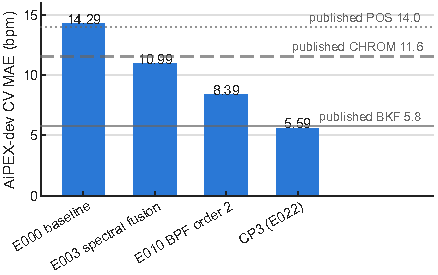
\includegraphics[width=\columnwidth]{figures/aipex_waterfall.pdf}
\caption{AiPEX-dev cross-validated MAE of the kept changes and the adopted CP3; published methods on all 88 videos for context.}
\label{fig:waterfall}
\end{figure}

\begin{table}[t]
\centering
\caption{AiPEX, one HR per video (bpm). CI: 95\,\% bootstrap over videos.}
\label{tab:aipex}
\begin{tabular}{@{}lcccc@{}}
\toprule
 & MAE [CI] & Median & Within 5 & Bias [LoA] \\
\midrule
CP2 dev (62, CV)        & 8.82 [7.0, 10.8] & 6.65 & 45\,\% & $+0.8$ [$-22$, $+24$] \\
CP2 test (26)           & 7.16 [5.2, 9.4] & 5.70 & 38\,\% & $-0.6$ [$-18$, $+17$] \\
\textbf{CP3 dev (62, CV)}  & \textbf{5.61 [4.6, 6.7]} & 4.99 & 50\,\% & $+0.4$ [$-14$, $+14$] \\
\textbf{CP3 test (26)}  & \textbf{5.96 [4.2, 7.9]} & 4.50 & 58\,\% & $+1.2$ [$-14$, $+16$] \\
\quad India / S.\ Leone (test) & 5.96 / 5.97 & & & \\
\midrule
\multicolumn{5}{@{}l}{Published, all 88~\cite{dasari2021bias}: BKF 5.8, CHROM 11.6, POS 14.0, Sph.\ mean 15.1, DeepPhys 15.5} \\
\bottomrule
\end{tabular}
\end{table}

\textbf{Test results.} On the 26 AiPEX-test subjects the frozen CP3 reaches \SI{5.96}{bpm} MAE (median \SI{4.50}{bpm},
58\,\% within \SI{5}{bpm}; Table~\ref{tab:aipex}), on par with the best published method on this dataset (BKF,
\SI{5.8}{bpm} on all 88 videos), with identical error for India and Sierra Leone (5.96 / \SI{5.97}{bpm}). Per-video
correlation with the reference remains low ($r=0.07$ on test, $0.30$ on dev): the references span only 66--\SI{93}{bpm} and
the estimates do not yet resolve between-subject differences within that range.

% sources: outputs/round1/c2_{dev,test}_CP3_*.csv (tools/c2_aipex.py); figure tools/make_c2_figure.py
\textbf{Skin tone (C2).} The individual typology angle ITA $=\mathrm{atan2}(L^*-50, b^*)\cdot180/\pi$ was computed from the
mean skin colour of the three crops (\texttt{rgb2lab}, sRGB/D65) and grouped as I--II, III--IV and V--VI. The tolerance
$\tau=\max(\SI{1}{bpm}, 0.25\cdot\mathrm{MAE})$ was pre-specified. No statistically significant difference in error between
ITA groups was detected (permutation test of the range of group MAEs: $p=0.73$ on dev, $p=0.72$ on test;
Fig.~\ref{fig:c2}). With $n=5/8/49$ (dev) and $2/5/19$ (test) videos the bootstrap CIs of the group deviations are wider
than $\pm\tau$, so the result is reported as inconclusive rather than as an absence of bias. Camera-derived ITA is a
lighting-dependent proxy, not a clinical Fitzpatrick rating: all five videos classified I--II on dev come from Sierra Leone,
which indicates illumination and white-balance effects.

\begin{figure}[t]
\centering
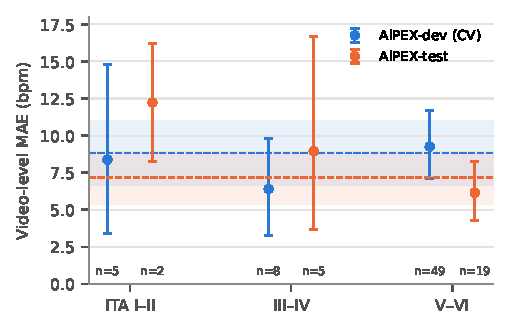
\includegraphics[width=0.9\columnwidth]{figures/c2_ita.pdf}
\caption{AiPEX MAE per ITA group (CP3) with 95\,\% bootstrap CIs; dashed lines: overall MAE, bands: $\pm\tau$.}
\label{fig:c2}
\end{figure}

% ================================================================================================
\section{Edge deployment and reproducibility}
\textbf{Web demonstrator.} A browser application implements the front end and an SNR-fusion signal chain in TypeScript:
MediaPipe landmarks, the ten patches, pixel selection and fusion run on the device in a Web Worker; a service worker caches
the application and model, so no network request is made after loading (C5, offline operation). It supports a
$320\times240$, 10\,fps mode, target designation by clicking (C3), occlusion display (C7), an ITA readout (C2), a whole-frame
low-light warning (C1), 1-Euro landmark smoothing and motion suppression. Its default signal core is a TypeScript port of the
frozen CP3 chain (the Butterworth coefficients match MATLAB to $10^{-12}$ and \texttt{filtfilt} uses MATLAB's edge handling).
Fed the same patch traces of three UBFC dev subjects, it reproduces the MATLAB window HRs exactly (0\,bpm difference in all 143
windows); in online mode (re-analysis of the newest 15\,s every second) all reported windows are within \SI{0.44}{bpm} of
MATLAB. One analysis step takes a median of \SI{13}{ms}. All 53 unit tests pass. \todo{browser timing, live-camera
validation against a pulse oximeter, screenshots.}

\textbf{Submission video encoding.} The pulse is only 0.1--1\,\% of the pixel intensity and is easily destroyed by
compression. MATLAB's \texttt{VideoWriter} MPEG-4 encoder saturates at about \SI{1.4}{Mbps} and raised the MAE on a
30\,s dev clip from 1.43 (lossless) to \SI{29.9}{bpm}. Encoding \texttt{target\_video.mp4} with x264 at CRF 4 with
adaptive quantisation, deblocking and psycho-visual tuning disabled (\SI{16}{Mbps}) keeps the pulse
(\SI{1.51}{bpm}, 100\,\% coverage) and remains readable by MATLAB.

\textbf{Reproducibility.} All results come from scripts in the repository; random seeds are fixed per video (the robust
motion estimate in the face tracker otherwise made results differ between runs); parameters, splits, the experiment log,
the changelog and both freeze tags are versioned.

% ================================================================================================
\section{Discussion and limitations}
\begin{itemize}
  \item On UBFC test the median subject is at \SI{1.2}{bpm}, but a single subject widens the limits of agreement; the
        superseded CP2 was better on this split, which we report rather than act on.
  \item AiPEX reaches the level of the best published method, but per-video correlation is low and AiPEX-test is not fully
        held out for CP3 (Section IV).
  \item Skin-tone results are inconclusive at these sample sizes, and ITA is a lighting-dependent proxy.
  \item Constraint results are from simulation on a small subset; real low-light and elderly data are not yet available.
  \item The organiser videos have no reference; no accuracy claim is made on them.
\end{itemize}

\section{Ethics and data statement}
We use the public UBFC-rPPG and AiPEX datasets under their licences, and the organiser's data under the competition
agreement. No faces from the organiser's data appear in this report. No new human-subject data were collected for Round~1.

\section*{Acknowledgment}
Face module and multi-face tracking: Sulojan Rajkumar; Kalman denoising and AiPEX evaluation: Thamilezai Ananthakumar;
SNR-fusion pipeline (adopted as the final signal chain) and skin-tone (C2) evaluation: Nadha Irshad; signal chain,
integration and web demonstrator: Muftee Mysan. \todo{contributions of Rajinthan Rameshkumar, John Praveen and Joshua
Kulasingham; supervisor; MathWorks licence.}

\bibliographystyle{IEEEtran}
\bibliography{refs}

\end{document}
